\section{WebGL}

\subsection{OpenGL Merkmale}

\begin{itemize} \setlength\itemsep{0em}
    \item Low Level Graphics API
    \item Verschiedene Platformen
    \item 1.0/2.0 Fixe Funktionspipeline
    \item Vorlage für WebGL
\end{itemize}

\subsection{Grafikpipeline}

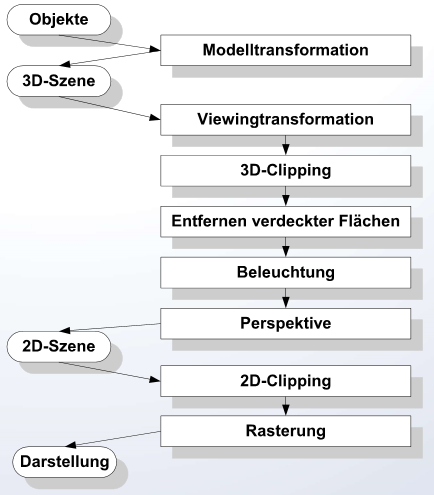
\includegraphics[width=0.4\textwidth]{assets/grafikpipline.png}

\subsection{Programmierbare Shaders}

\textit{
    Shaders werden für die Berechnung der zu zeichnenden
    Objekte verwendet. Das Programm wird direkt auf der Grafikkarte
    ausgeführt.
}

\subsubsection{Vertex Processing / Vertex Shader}

\textit{
    Berechnen der \textbf{Positionen} der Vertexe (Punkte) und
    Werte für den folgenden Fragmentshader.
}

\subsubsection{Fragment Processing / Fragment Shader}

\textit{
    Berechnet die \textbf{Farbe} der einzelnen Pixel.
}

\subsection{Datenfluss}

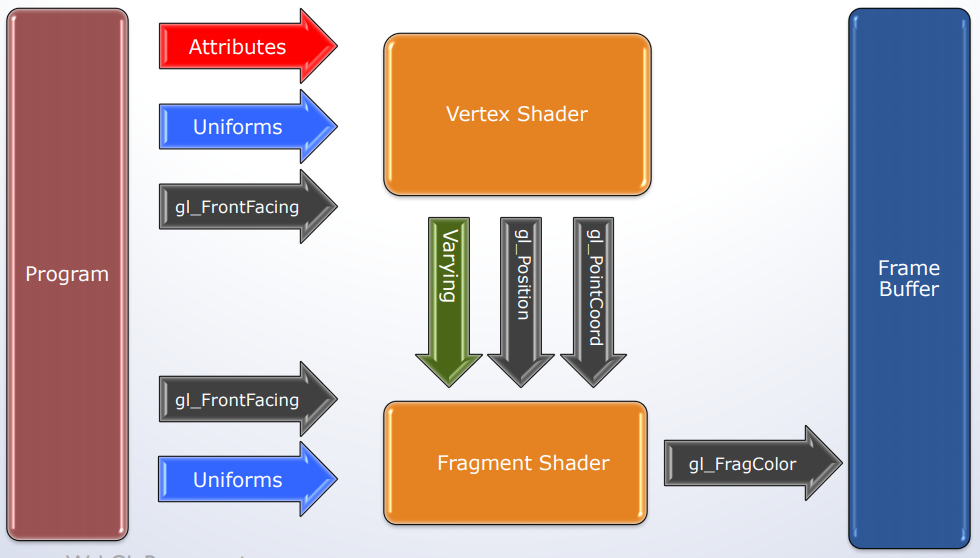
\includegraphics[width=0.5\textwidth]{assets/dataprocessing.png}

\subsection{Attribute und Uniform Variablen mit Shaders verbinden}

\begin{enumerate}
	\item Attribute \\
	\texttt{ctx.aVertexPositionId = gl.getAttribLocation(ctx.shaderProgram, "aVertexPosition")}
	
	\item Uniform \\
	\texttt{ctx.uColorId = gl.getUniformLocation(ctx.shaderProgram, "uColor"))}
	
\end{enumerate}

\subsection{Attribut Variablen und Buffer definieren}

\textbf{Erzeugen}

\begin{enumerate}
    \item Buffer erzeugen \\
    \texttt{var buffer = gl.createBuffer()}
    
    \item Array Buffer auf Buffer setzen \\
    \texttt{gl.bindBuffer(gl.ARRAY\_BUFFER, buffer)}
    
    \item Daten füllen \\
    \texttt{gl.BufferData(gl.ARRAY\_BUFFER, new Float32Array(vertices), gl.STATIC\_DRAW)}
\end{enumerate}

\textbf{Zeichnen}

\begin{enumerate}
    \item Buffer binden
    \item Attribut und/oder uniform setzen \\
    \texttt{gl.vertexAttribPointer(index, size, type, normalized, stride, offset)} \\
    z.B. \texttt{gl.vertexAttribPointer(ctx.aVertexPositionId, 2, gl.FLOAT, false, 0, 0)}
    
    \item Attribut als Array setzen \\
    \texttt{gl.enableVertexAttribArray(index)}
    
    \item Zeichnen \\
    \texttt{gl.drawArrays(mode, first, count)}
\end{enumerate}